\documentclass[conference]{IEEEtran}

\usepackage[utf8]{inputenc}
\usepackage[T1]{fontenc}
\usepackage{amsmath,amssymb}
\usepackage{booktabs,array,multirow,tabularx}
\usepackage{graphicx}
\usepackage{balance}
\usepackage{xcolor}
\usepackage{listings}
\usepackage{tikz}
\usetikzlibrary{arrows.meta,positioning,shapes.geometric,fit,calc}
\usepackage[hidelinks]{hyperref}
\usepackage{url}

\newcommand{\code}[1]{\texttt{#1}}
\newcolumntype{Y}{>{\raggedright\arraybackslash}X}
\newcolumntype{C}[1]{>{\centering\arraybackslash}p{#1}}

\lstdefinestyle{py}{
  language=Python,
  basicstyle=\ttfamily\scriptsize,
  keywordstyle=\bfseries,
  commentstyle=\itshape\color{gray},
  numbers=none,
  frame=single,
  framerule=0.3pt,
  captionpos=b,
  aboveskip=4pt,
  belowskip=2pt,
  belowcaptionskip=4pt,
  breaklines=true,
  xleftmargin=2pt,
  xrightmargin=2pt,
  columns=fullflexible,
  keepspaces=true,
  showstringspaces=false
}
\lstset{style=py}

\begin{document}

\title{TCP-Based Multi-Client LAN Messaging: A Survey of Transport, Framing, Concurrency and Security, and LANChat-H, an Implemented and Measured Dependency-Light Reference Design}

\author{
\IEEEauthorblockA{%
\begin{tabular}{C{2.1in}C{2.1in}C{2.1in}}
1\textsuperscript{st} Harish Goud B & 2\textsuperscript{nd} Revanth Reddy Lingala & 3\textsuperscript{rd} Saarthak Manocha \\[2pt]
\textit{Dept. of Information Technology} & \textit{Dept. of Information Technology} & \textit{Dept. of Information Technology} \\
\textbf{\textit{Chaitanya Bharathi Institute of Technology}} & \textbf{\textit{Chaitanya Bharathi Institute of Technology}} & \textbf{\textit{Chaitanya Bharathi Institute of Technology}} \\
Hyderabad, India & Hyderabad, India & Hyderabad, India \\
harishgoudbit@cbit.ac.in & revanth252017@gmail.com & saarthakmanocha10@gmail.com \\
\end{tabular}%
}
}

\maketitle

\begin{abstract}
A local-area chat application looks trivial from the user's side, yet it forces a designer to solve several networking and security problems at once: recovering message boundaries from a byte stream, serving many clients concurrently, distributing each message to a group, surviving abnormal disconnections, and deciding whom to trust. The literature that addresses these problems is large but fragmented: transport standards describe the byte stream, server-architecture research compares threads with events, messaging standards such as IRC, XMPP, MQTT and WebSocket each fix one design point, and work on reliable groups and secure messaging studies guarantees far stronger than a small system needs. This paper surveys that literature through the lens of a concrete artifact, LANChat-H, a chat system whose core uses only the Python standard library. One TCP server runs a handler thread and a bounded outbound queue with a writer thread per client; messages travel in length-prefixed frames carrying either plain text or versioned JSON events; connections are protected by TLS with trust-on-first-use certificate pinning, memory-hard password hashing, role checks, login lockout and rate limits; history is stored in SQLite; files move over separate, ticket-authorised connections and are verified by SHA-256; and administrative actions are recorded in a hash-chained audit log. On a single laptop over loopback, median delivery latency stayed between 2.7 and 5.8 ms for up to 100 receivers; when one receiver stopped reading, a sequential-relay baseline stopped delivering to all others after about 232 messages whereas the bounded-queue server delivered all 6000 of 6000; and the code base is covered by 343 automated tests and 205 scripted checks that drive the real window and the terminal client. Key management for end-to-end encryption is implemented; encrypting message bodies, forward secrecy and an asynchronous server variant remain future work.
\end{abstract}

\begin{IEEEkeywords}
TCP, socket programming, LAN chat, message framing, length prefix, concurrent server, thread-per-client, head-of-line blocking, TLS, trust on first use, audit log, end-to-end encryption
\end{IEEEkeywords}

%======================================================================
\section{Introduction}
%======================================================================
A chat program rarely needs to do anything clever to be useful. Two people type, and each sees what the other typed. Underneath that simple behaviour, however, sits a stack of decisions that every networked application has to make. The server must accept connections and remember who is connected. It must turn a continuous stream of bytes back into the individual messages that were sent. It must handle many clients at the same time without letting shared state become corrupted. It must deliver each message to everyone else in the room, and it must notice and clean up after a client that vanishes without saying goodbye.

TCP is the natural transport, because it offers a reliable, ordered, full-duplex byte stream \cite{rfc9293,rfc793}. The important word is \emph{byte}. The current TCP specification deliberately exposes a stream rather than a sequence of records, so a single \code{send()} on one side does not correspond to a single \code{recv()} on the other \cite{rfc9293,stevens}. A message can arrive split across several reads, and several messages can arrive glued together in one read. Any chat protocol built directly on sockets therefore has to define its own message boundaries.

Several research and standards communities have worked on parts of this problem, each from a different angle. One community specifies the transport itself: reliability, flow control and congestion control \cite{rfc9293,jacobson,rfc5681}. A second community compares ways of serving many connections, from threads and processes to event loops and staged pipelines \cite{flash,seda,vonbehren,ousterhout,kegel}. A third community defines complete messaging protocols, among them IRC, XMPP, MQTT and WebSocket \cite{rfc1459,rfc6120,mqtt5,rfc6455}. A fourth studies what it takes to give a group of processes consistent delivery in the presence of failures \cite{birman87,birman93,eugster}. Finally, work on secure messaging explains what an eavesdropper or an impersonator can do to a plaintext channel and what the remedies cost \cite{rfc8446,unger,signal}.

What stands out when these bodies of work are placed side by side is how little they meet. A protocol standard tells a reader what a frame looks like, but not how a small server should schedule its handlers. A server-architecture paper compares throughput, but usually on web workloads rather than on a long-lived, many-to-many chat session. A group-communication paper reasons about failure models that a teaching system never approaches. Textbooks do walk through sockets and threads \cite{stevens,tanenbaum,kurose}, but they present them as separate exercises, and a reader who wants to see framing, concurrency, broadcast and shutdown interacting in one short program has to assemble that picture alone.

This is the gap that motivates the paper. Rather than choosing one of these threads to specialise in, we survey them together, anchored to one concrete artifact: a Python chat system whose core is built with nothing beyond the standard library \cite{pysocket,pythreading}, which we use as a running case. The system began as a minimal threaded relay and was hardened in stages; the version described here is called LANChat-H (H for hardened). The contributions are:
\begin{enumerate}
  \item a thematic survey of the transport, framing, concurrency, messaging-protocol, reliability, trust and security literature relevant to a small TCP chat system;
  \item a comparative analysis of the reviewed approaches and the reference implementation, together with the design decisions they represent;
  \item a description of LANChat-H stated precisely from its source code, including what it enforces and what it deliberately omits;
  \item an explicit research gap, and the staged hardening path by which the implementation addresses it; and
  \item a reproducible evaluation: protocol and security tests, fan-out latency, a head-of-line-blocking experiment against a sequential-relay baseline, file-transfer speed and per-operation security costs, with the code, tests and scripts published online \cite{lanchatrepo} and the limits of the measurements stated.
\end{enumerate}
Section~II gives the technical background. Section~III reviews and compares the literature. Section~IV states the research gap. Section~V describes LANChat-H. Section~VI presents the evaluation, Section~VII discusses limits and future work, and Section~VIII concludes.

%======================================================================
\section{Background}
%======================================================================

\subsection{TCP as a Byte Stream}
TCP establishes connection state before any data moves, numbers every byte so that lost segments can be retransmitted and out-of-order segments reassembled, and uses a window to stop a fast sender from overwhelming a slow receiver \cite{rfc793,rfc9293}. Congestion control, introduced by Jacobson and later standardised, limits how quickly a sender injects data into the network through slow start, congestion avoidance, fast retransmit and fast recovery \cite{jacobson,rfc5681}. Together these mechanisms give an application an ordered, loss-free byte stream.

They do not give it more than that. TCP does not know about users, rooms or messages, it does not persist anything across a process crash, and it does not confirm that a particular chat participant actually read a particular line. This is an instance of the end-to-end argument: functions that only the application can implement completely, such as message boundaries or delivery confirmation to a person, cannot be delegated wholesale to the lower layer \cite{saltzer}.

\subsection{Connection Failure and Liveness}
A TCP connection can end cleanly, with an exchange of FIN segments, or it can fail through a reset, a timeout, a crashed process, a dropped interface or a network partition. An application normally learns about failure when a read returns end-of-stream, when a send or receive raises an exception, or when a liveness policy expires. TCP keep-alive is optional and off by default; the host-requirements standard requires that it be configurable and warns that a single unanswered probe is not proof that the peer is gone \cite{rfc1122}. In practice this means that explicit quit commands and exception handling handle the common case, whereas noticing an unplugged laptop quickly needs application-level timeouts or heartbeat messages.

\subsection{Why Framing Is Mandatory}
Because TCP segmentation is independent of application writes, a receiver cannot rely on read boundaries. Four framing strategies dominate practice, summarised in Table~\ref{tab:framing}. \emph{Fixed-size} records are trivial to parse but waste space and cannot carry variable payloads. \emph{Delimiter}-based framing, used by line-oriented protocols such as IRC, is readable but needs an escaping rule whenever the delimiter can occur inside the data \cite{rfc1459}. \emph{Length-prefixed} framing announces the payload size before the payload, so a receiver reads exactly that many bytes; it is binary-safe and precise, at the price of having to validate the announced length. \emph{Self-describing} formats, such as the XML streams of XMPP, carry structure inside the data but still depend on an outer mechanism to find where one unit ends \cite{rfc6120}. WebSocket and MQTT both use length information in binary headers \cite{rfc6455,mqtt5}.

\begin{table}[t]
\centering
\caption{Application-Layer Framing Alternatives}
\label{tab:framing}
\footnotesize
\begin{tabularx}{\columnwidth}{@{}l Y Y@{}}
\toprule
\textbf{Method} & \textbf{Advantage} & \textbf{Limitation} \\
\midrule
Fixed size & Trivial parsing & Wasted space; inflexible \\
Delimiter & Human-readable; simple for lines & Escaping and delimiter collision \\
Length prefix & Binary-safe; exact; variable size & Length must be validated \\
TLV & Extensible typed fields & Larger parser and schema \\
Self-describing & Rich structure (XML/JSON) & Encoding overhead; needs outer framing \\
\bottomrule
\end{tabularx}
\end{table}

For a stream of UTF-8 text \cite{rfc3629}, a four-byte unsigned length in network byte order followed by the encoded payload is compact and easy to test. Python's \code{struct} module defines the \code{!} format prefix as network (big-endian) order with standard sizes, so \code{"!I"} is an interoperable four-byte header \cite{pystruct}. The receiver must loop until the requested number of bytes has accumulated or the peer closes, because a single \code{recv()} may return fewer bytes than asked for. Fig.~\ref{fig:framing} shows the idea, and Listing~\ref{lst:frame} shows the code used by the reference implementation.

\begin{figure}[t]
\centering
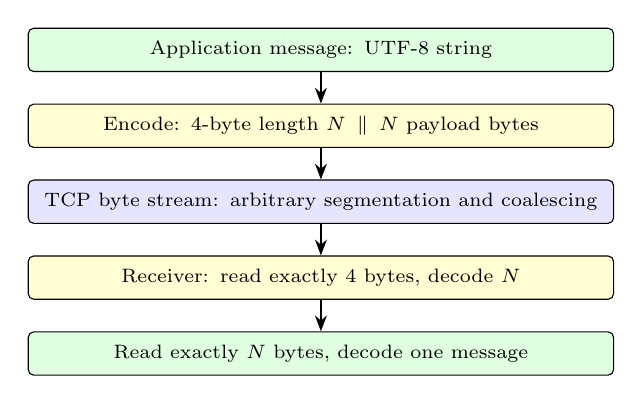
\begin{tikzpicture}[
  box/.style={draw, rounded corners=2pt, font=\scriptsize, minimum height=5.5mm, text width=7.2cm, align=center},
  arr/.style={-{Stealth[length=2mm]}, thick}
]
\node[box, fill=green!12] (a) {Application message: UTF-8 string};
\node[box, fill=yellow!18, below=4mm of a] (b) {Encode: 4-byte length $N$ \,$\Vert$\, $N$ payload bytes};
\node[box, fill=blue!10, below=4mm of b] (c) {TCP byte stream: arbitrary segmentation and coalescing};
\node[box, fill=yellow!18, below=4mm of c] (d) {Receiver: read exactly 4 bytes, decode $N$};
\node[box, fill=green!12, below=4mm of d] (e) {Read exactly $N$ bytes, decode one message};
\draw[arr] (a)--(b); \draw[arr] (b)--(c); \draw[arr] (c)--(d); \draw[arr] (d)--(e);
\end{tikzpicture}
\caption{Length-prefixed framing over a TCP byte stream.}
\label{fig:framing}
\end{figure}

\begin{lstlisting}[caption={Framing logic of the reference implementation (\texttt{protocol.py}, condensed).},label={lst:frame},float=t]
MAX_MESSAGE_BYTES = 4096

def send_message(conn, message):
    payload = message.encode("utf-8")
    if len(payload) > MAX_MESSAGE_BYTES:
        raise ValueError("message is too large")
    conn.sendall(struct.pack("!I", len(payload)) + payload)

def receive_message(conn):
    header = _receive_exactly(conn, 4)
    if header is None:
        return None            # peer closed
    (length,) = struct.unpack("!I", header)
    if length == 0 or length > MAX_MESSAGE_BYTES:
        raise ValueError("invalid message length")
    payload = _receive_exactly(conn, length)
    if payload is None:
        return None
    return payload.decode("utf-8")
\end{lstlisting}

\subsection{Concurrency Models for Servers}
A chat server holds many connections open for a long time, and most of the time each one is idle. Four models are usually contrasted. \emph{Thread-per-client} gives each connection a sequential control flow that is easy to read and debug, at the cost of one stack and one scheduling entity per client. A \emph{thread pool} bounds the number of workers but adds queueing and makes long-lived connections awkward. An \emph{event loop} multiplexes many connections on few threads using readiness notification, which scales further but forces the programmer to express each connection as a state machine \cite{kegel,krohn}. \emph{Staged} architectures split a service into event-driven stages joined by explicit queues with dynamic resource control \cite{seda}. The debate between threads and events is old and unresolved: Ousterhout argued that threads are the wrong abstraction for most purposes, von Behren \emph{et al.} argued that the objections are really objections to particular thread implementations, and Lee described the difficulty of reasoning about shared-memory threads \cite{ousterhout,vonbehren,lee}.

\subsection{Group Delivery and Topology}
Delivering one message to many recipients can be done in several ways. A central server can relay by repeated unicast, sending a separate copy on each connection. Peer-to-peer designs remove the relay but introduce membership, connection-count and consistency problems. IP multicast sends one datagram to a group, but it uses datagram semantics, which moves loss recovery, ordering and membership back to the application \cite{rfc1112}. Broker-based publish--subscribe decouples senders and receivers in space, time and synchronisation \cite{eugster}. Repeated unicast is not Ethernet broadcast or IP multicast: every recipient has an independent TCP connection with its own flow-control window and failure state.

\subsection{Security Considerations}
A trusted LAN reduces deployment effort but is not a security mechanism. On a plaintext channel, any reachable host can connect, choose any name, inject messages, and read traffic. TLS~1.3 protects a client--server channel against eavesdropping, tampering and forgery and can authenticate the server with a certificate \cite{rfc8446}. It does not authenticate individual users, and the server still sees plaintext after decryption. End-to-end secrecy between users needs a different construction, such as the Double Ratchet used by Signal, which provides forward secrecy and post-compromise security \cite{signal,cohngordon}. Unger \emph{et al.} give a systematic comparison of secure-messaging designs \cite{unger}.

Three further mechanisms matter for a small multi-user server. First, trust in a self-signed server certificate can be established on first use and then pinned, the model that SSH uses for host keys \cite{rfc4251}; it protects every later connection but not the first. Second, passwords should be stored only as salted, memory-hard hashes such as scrypt \cite{rfc7914}, and online guessing should be throttled, as recommended for authentication systems generally \cite{nist63b}. Third, an audit log whose entries are chained by hashes makes later alteration detectable \cite{schneier99,crosby09}.

%======================================================================
\section{Literature Review}
%======================================================================
Rather than reviewing sources one by one, it is more useful to group them by the design question they answer. Table~\ref{tab:comparison} compares the approaches discussed below, and the reference implementation, on the properties most relevant to a small LAN chat system.

\begin{table*}[t]
\centering
\caption{Comparative Analysis of Reviewed Approaches}
\label{tab:comparison}
\scriptsize
\renewcommand{\arraystretch}{1.1}
\begin{tabularx}{\textwidth}{@{}>{\raggedright\arraybackslash}p{2.6cm} Y Y Y Y Y Y@{}}
\toprule
\textbf{Approach} & \textbf{Transport} & \textbf{Framing} & \textbf{Topology} & \textbf{Security} & \textbf{Persistence} & \textbf{Key limitation for a small teaching system} \\
\midrule
IRC \cite{rfc1459,rfc2812} & TCP & CRLF lines, 512-byte limit & Server network & None in base spec & None & Text-only framing; limits fixed by the spec \\
XMPP \cite{rfc6120,rfc6121} & TCP & XML stream & Federated client--server & SASL and TLS & Via extensions & Heavy parser; large specification surface \\
MQTT 5.0 \cite{mqtt5} & TCP (optionally TLS) & Binary header, variable length & Broker pub/sub & Optional; credentials in CONNECT & Sessions and QoS & Needs a broker; more machinery than a chat room needs \\
WebSocket \cite{rfc6455} & TCP after HTTP upgrade & Length-carrying frames; client masking & Client--server & TLS via \code{wss} & None & Needs an HTTP handshake and a framework \\
Signal / Double Ratchet \cite{signal,cohngordon} & Any & Not specified & Relayed & End-to-end & Server-dependent & Cryptographic design, not a transport or server design \\
FTP \cite{rfc959} & TCP, separate control and data connections & Commands as text lines; data as a raw stream & Client--server & None in base spec & Files only & Predates TLS; no chat, presence or history \\
Flash \cite{flash} & TCP (web) & HTTP & Client--server & N/A & N/A & Web workload; compares process, thread and event models \\
SEDA \cite{seda} & TCP (services) & Application-defined & Staged pipeline & N/A & N/A & Targets far larger loads than a classroom chat \\
Threads vs.\ events \cite{ousterhout,vonbehren,krohn} & TCP & N/A & N/A & N/A & N/A & Position papers, not chat-specific \\
Reliable groups \cite{birman87,birman93} & Reliable channels & N/A & Process groups & N/A & Varies & Guarantees far beyond a demonstration system \\
\textbf{LANChat-H (this work)} & \textbf{TCP + TLS} & \textbf{4-byte length + text or JSON events} & \textbf{Central relay} & \textbf{TLS with pinning, scrypt, roles, audit} & \textbf{SQLite} & \textbf{Single server; message bodies not yet end-to-end encrypted (Sec.~VII)} \\
\bottomrule
\end{tabularx}
\end{table*}

\textbf{Complete messaging protocols.} IRC was the first widely deployed text chat protocol on TCP. Its base specification frames messages as lines ending in carriage return and line feed, limited to 512 characters, and connects servers in a network so that users on different servers can talk to each other \cite{rfc1459,rfc2812}. The design is easy to implement by hand, which explains its longevity, but the delimiter approach forces every reader to agree on how to handle over-long or malformed lines. XMPP takes the opposite direction: it defines a long-lived XML stream over TCP with negotiation of TLS and SASL authentication, and a separate specification adds rosters and presence for instant messaging \cite{rfc6120,rfc6121}. That richness is precisely what makes it heavy for a small system. MQTT~5.0 places a broker between publishers and subscribers and adds quality-of-service levels, sessions and a compact binary header \cite{mqtt5}. WebSocket adds an HTTP-compatible opening handshake and then exchanges length-carrying frames, which makes it the natural route to browser clients \cite{rfc6455}. All four solve interoperability and deployment problems that a command-line demonstration deliberately sidesteps.

\textbf{Server-architecture research.} Pai, Druschel and Zwaenepoel compared multi-process, multi-threaded, single-process event-driven and asymmetric event-driven designs in the Flash web server and showed that architecture materially changes throughput and blocking behaviour \cite{flash}. SEDA proposed decomposing a service into stages linked by bounded queues, with dynamic controllers that keep the system stable under overload \cite{seda}. Position papers on both sides of the threads-versus-events debate followed \cite{ousterhout,vonbehren,lee}, and Krohn \emph{et al.} argued that event-driven code can be written with a structure close to threaded code \cite{krohn}. The C10K discussion collected the operating-system techniques needed to serve ten thousand simultaneous connections \cite{kegel}. What these works share is that their target workloads are much larger and more heterogeneous than a room of a few terminals. They justify an architectural boundary, meaning the point at which thread-per-client stops being adequate, without proving that threads are the wrong choice below it.

\textbf{Group communication and reliability.} Birman and Joseph's work on virtual synchrony and the later process-group approach show what \emph{reliable} group delivery means when processes can fail: members agree on group views and on the order in which messages are delivered relative to membership changes \cite{birman87,birman93}. Eugster \emph{et al.} survey publish--subscribe and classify it by how it decouples producers and consumers \cite{eugster}. A chat server that relays by repeated unicast provides none of these guarantees. A message accepted by the server can reach some clients before another connection fails, and there is no acknowledgement set, replay or globally stable order. Distinguishing this from transport reliability is important, because TCP's reliability is easily mistaken for delivery reliability.

\textbf{Secure messaging.} TLS~1.3 secures the channel \cite{rfc8446}, and the secure-messaging literature separates transport security, user authentication, authorisation, and end-to-end secrecy as distinct layers \cite{unger}. Signal's Double Ratchet shows how end-to-end secrecy with forward secrecy can be combined with an untrusted relay \cite{signal,cohngordon}. These layers are additive, and a system can adopt them in stages. The same layering applies to groups: the X3DH key agreement gives asynchronous contact set-up between parties that need not be online together \cite{x3dh}, and the Messaging Layer Security protocol addresses efficient group key management with member addition and removal \cite{rfc9420}. Both rest on the same primitives that are available in widely reviewed libraries: X25519 key agreement \cite{rfc7748}, Ed25519 signatures \cite{rfc8032}, HKDF \cite{rfc5869} and ChaCha20-Poly1305 \cite{rfc8439}.

\textbf{Credentials, trust establishment and audit.} Small systems usually treat accounts as an afterthought. Standards guidance on authentication recommends salted, memory-hard password hashing, a minimum length with a check against common passwords, and limits on repeated failed attempts \cite{nist63b,rfc7914}. For servers with self-signed certificates, SSH's trust-on-first-use host-key model is the most widely deployed precedent \cite{rfc4251}. For accountability, tamper-evident logging work shows that chaining each entry's hash to its predecessor lets an auditor detect modification, deletion or insertion, with a separate commitment to the newest entry needed to detect truncation \cite{schneier99,crosby09}. These ideas appear in operating systems and services, but rarely in a teaching-scale chat server where all of them can be read together.

\textbf{Discovery and bulk transfer.} On a LAN, services are normally found with multicast DNS and DNS-based service discovery \cite{rfc6762,rfc6763}; small programs often use a custom UDP broadcast instead, which is simpler but limited to one broadcast domain. For files, FTP established the pattern of a control connection for commands and a separate data connection for bytes \cite{rfc959}, so that a large transfer never blocks or overflows the command channel. Modern chat protocols that carry media over their message channel must either fragment it or rely on a side channel for the same reason.

\textbf{Foundational texts.} Stevens' treatment of the sockets API and the standard networking textbooks remain the main sources for how a program actually uses TCP \cite{stevens,tanenbaum,kurose}.

Read together, these groups trace a fairly clean progression: from byte-stream transport, to explicit message framing, to concurrent servers, to full messaging protocols, and finally to reliable and secure group communication. What none of them does individually is present a compact, dependency-free system in which all of these decisions interact and can be inspected and measured at once.

%======================================================================
\section{Research Gap}
%======================================================================
Reading Table~\ref{tab:comparison} left to right, every reviewed approach is strong in the columns it was designed for and silent elsewhere. The remainder of this section explains why closing the gaps is a matter of design, not of adding one more feature.

\textbf{Framing, concurrency and shutdown are studied separately.} Protocol standards specify frames, architecture papers compare schedulers, and textbooks teach sockets and threads as independent exercises. In a real chat server they interact: a handler thread blocks inside a read while another thread wants to shut the server down, a broadcast iterates a client table while another handler removes an entry, and a half-received frame is abandoned when a peer disconnects mid-message. Few sources examine these interactions in a system small enough to read in one sitting.

\textbf{Sequential broadcast has a head-of-line risk.} When a handler sends a message to every recipient in turn, a slow receiver whose send buffer is full can delay delivery to every recipient after it. Per-client outbound queues with writer workers, bounded queues with a disconnect-or-drop policy, or non-blocking writes isolate slow consumers. This is well known in large systems \cite{seda}, but it is rarely shown in a teaching-scale implementation together with the code and tests that demonstrate the problem.

\textbf{Liveness detection is left to defaults.} Because TCP keep-alive is optional and off by default \cite{rfc1122}, a suspended laptop or an unplugged cable can leave a connection half-open for a long time. Explicit exit and exception cleanup cover normal termination, but abnormal termination needs a heartbeat or timeout that is seldom included in small examples.

\textbf{Security is either absent or arrives all at once.} Simple demonstrations are plaintext with no identity; production systems bring TLS, accounts and end-to-end encryption together \cite{rfc8446,unger,signal}. The intermediate steps, such as wrapping sockets with the standard \code{ssl} module and adding a name-uniqueness rule, are rarely presented as a staged path with a clear statement of what each stage does and does not protect.

\textbf{Evaluation is anecdotal.} Very few small messaging examples come with a protocol-correctness test that fragments and coalesces frames, or with a measurement method for latency and fan-out cost. Without one, no claim about when thread-per-client stops being adequate can be checked.

LANChat-H (Section~V) is built around the premise that these gaps share one root cause: transport, framing, concurrency, delivery and security are presented as separate problems, when in a chat system they are stages of one path that must agree on message size limits, lifecycle and failure handling. Section~VI reports what happens when that path is built and measured.

%======================================================================
\section{LANChat-H: The Reference Implementation}
%======================================================================
LANChat-H is the case-study system. It began as a minimal command-line relay (a TCP server, one thread per client, a four-byte length prefix and plaintext broadcast, with three tests) and was extended in stages, each independently testable. This section states what the current source code does; Section~VI measures it. The core uses only the Python standard library \cite{pysocket,pythreading,pystruct,pyssl}. The standard-library modules \code{sqlite3} and \code{hashlib} supply storage and scrypt \cite{pysqlite,pyhashlib}, and \code{tkinter} supplies the desktop window. Three third-party packages are optional: \code{cryptography} for end-to-end key management, Pillow for some picture previews and \code{sounddevice} for voice recording.

\subsection{Architecture}
Fig.~\ref{fig:arch} shows the structure. The server owns membership, persistence and policy; clients are thin. In total the non-graphical code is about 4,400 lines in 20 modules, the window about 3,900 lines in seven modules, and key management about 400 lines. Table~\ref{tab:mapping} maps modules to the concepts surveyed earlier.

\begin{figure}[t]
\centering
\resizebox{\columnwidth}{!}{%
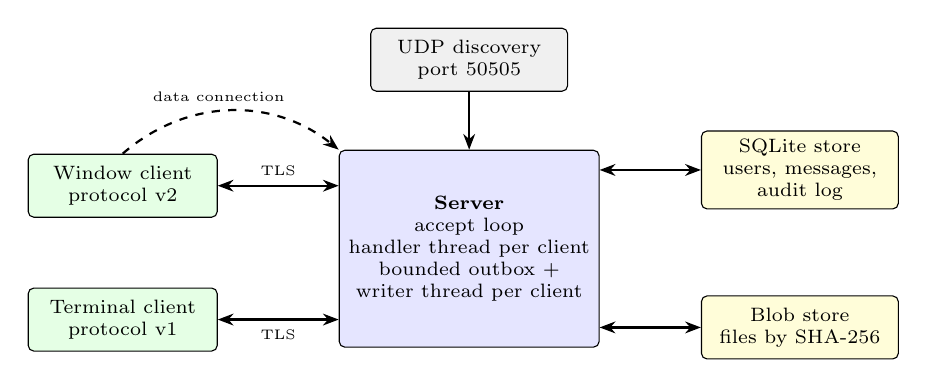
\begin{tikzpicture}[
  box/.style={draw, rounded corners=2pt, font=\scriptsize, align=center, minimum height=8mm, inner sep=3pt},
  arr/.style={{Stealth[length=2mm]}-{Stealth[length=2mm]}, thick},
  one/.style={-{Stealth[length=2mm]}, thick}
]
\node[box, fill=green!10, minimum width=2.4cm] (gui) at (0,1.0) {Window client\\protocol v2};
\node[box, fill=green!10, minimum width=2.4cm] (term) at (0,-0.7) {Terminal client\\protocol v1};
\node[box, fill=blue!10, minimum width=3.3cm, minimum height=2.5cm] (srv) at (4.4,0.2) {\textbf{Server}\\accept loop\\handler thread per client\\bounded outbox +\\writer thread per client};
\node[box, fill=yellow!15, minimum width=2.5cm] (db) at (8.6,1.2) {SQLite store\\users, messages,\\audit log};
\node[box, fill=yellow!15, minimum width=2.5cm] (blob) at (8.6,-0.8) {Blob store\\files by SHA-256};
\node[box, fill=gray!12, minimum width=2.5cm] (udp) at (4.4,2.6) {UDP discovery\\port 50505};
\draw[arr] (gui)--node[above,font=\tiny]{TLS}(srv.west |- gui);
\draw[arr] (term)--node[below,font=\tiny]{TLS}(srv.west |- term);
\draw[arr] (srv.east |- db)--(db);
\draw[arr] (srv.east |- blob)--(blob);
\draw[one] (udp)--(srv);
\draw[one, dashed] (gui.north) to[bend left=40] node[above,font=\tiny,pos=0.45]{data connection} (srv.north west);
\end{tikzpicture}}
\caption{Architecture of LANChat-H. Both client kinds hold one TLS connection to a central relay; file bytes use a second, short-lived data connection authorised by a ticket from the first.}
\label{fig:arch}
\end{figure}

\begin{table*}[t]
\centering
\caption{Implementation Mapping and Honest Scope}
\label{tab:mapping}
\footnotesize
\begin{tabularx}{\textwidth}{@{}>{\raggedright\arraybackslash}p{3.6cm} >{\raggedright\arraybackslash}p{2.9cm} Y Y@{}}
\toprule
\textbf{Component} & \textbf{Concept} & \textbf{Role in the system} & \textbf{Boundary / not provided} \\
\midrule
\code{protocol.py}, \code{events.py} & Record recovery; typed events & 4-byte network-order length, exact-read loop, 4096-byte limit; JSON events with a type field, plus a renderer that turns any event into a plain line for old clients & No acknowledgements or sequence numbers on the wire \\
\code{server.py}, \code{server\_admin.py}, \code{server\_keys.py} & Accept, membership, fan-out, policy & Handler thread and bounded outbox with writer thread per client; handshake; history, search, pins; ticketed file transfer; admin and key-directory events & Single server; no failover; one thread per client \\
\code{store.py}, \code{accounts.py}, \code{permissions.py} & Persistence, credentials, roles & SQLite with six numbered migrations, FTS5 search with \code{LIKE} fallback; scrypt hashes; admin, member and guest roles checked on the server & One connection behind a lock; not a clustered database \\
\code{security.py}, \code{audit.py} & Abuse resistance; accountability & Lockout with backoff, token-bucket rate limits, connection and sign-up caps, password rules; hash-chained audit log & In-memory counters reset on restart \\
\code{storage.py}, \code{transfer.py} & Bulk transfer & Content-addressed blob store, name sanitising, blocked types, streaming SHA-256 verification & Files are not encrypted at rest on the host \\
\code{chat\_core.py}, \code{certs.py}, \code{discovery.py} & Client handshake, TLS trust, discovery & Login, certificate pinning by SHA-256 fingerprint, self-signed certificate creation, UDP broadcast discovery & Discovery works within one broadcast domain \\
\code{e2ee.py}, \code{keystore.py} & End-to-end key management & Identity keys, passphrase-wrapped key file, recovery code, safety numbers, pinned contacts, sealed-message primitive & Message bodies are not yet sent encrypted (Sec.~VII) \\
\code{gui\_*.py}, \code{client.py}, \code{chat.py}, \code{admin\_cli.py} & Interface & Desktop window, terminal client, single launcher, offline admin tool & Terminal client lacks edits, reactions, search and pictures \\
\bottomrule
\end{tabularx}
\end{table*}

\subsection{Framing, Protocol Versions and Compatibility}
Every message in both directions is a four-byte big-endian length followed by UTF-8 text, as in Listing~\ref{lst:frame}; zero-length and over-long frames close the connection. Two protocol versions share this framing. Version~1 carries plain text lines and is what the terminal client speaks. Version~2 carries one JSON object per frame with a type field (message, edit, delete, reaction, typing, presence, read marker, pin, search, history page, upload, download and so on); a version-2 client announces itself with a JSON hello in the username step, and the server detects the version from the first character. For version-1 clients the server renders every event as the line they have always seen, and returns nothing for events a terminal cannot show, so new features were added without breaking the old client. Message text is limited to 3400 bytes so that the JSON envelope always fits one frame.

\subsection{Concurrency and Delivery}
Each connection has a handler thread that reads requests and a writer thread that is the only code writing to that socket. Delivering a message means placing it on every recipient's bounded outbound queue (default 100 entries) without waiting. If a queue fills, the client is not keeping up and is disconnected; it can reconnect and replay history from the database. This is the Stage~1 isolation of slow receivers described in the original design, and Section~VI measures its effect. The welcome and history are written directly before the writer thread starts, so they arrive first and in order. Clients send a ping every ten seconds and the server drops a connection silent for thirty. A user name may be signed in once; a saved sign-in may take over a stale connection.

\subsection{Security Design}
Table~\ref{tab:security} lists each threat with its control; the controls are in code and covered by tests (Section~VI).

\begin{table*}[t]
\centering
\caption{Threats and Controls in LANChat-H}
\label{tab:security}
\footnotesize
\begin{tabularx}{\textwidth}{@{}>{\raggedright\arraybackslash}p{3.6cm} Y@{}}
\toprule
\textbf{Threat} & \textbf{Control} \\
\midrule
Reading or altering traffic & TLS (1.2 or newer) on chat and data connections. The host creates a self-signed certificate once. \\
Impersonating the server & Trust on first use: the client shows the certificate's SHA-256 fingerprint, pins the certificate after approval and refuses a different one later. Host name checking is off because LAN addresses change; the pinned certificate authenticates the server. \\
Stolen account database & Passwords stored only as salted scrypt hashes ($n=2^{14}$, $r=8$, $p=1$, 32-byte output) with constant-time comparison. \\
Password guessing & Five wrong passwords lock a name from an address for 30 s, doubling to 15 min; one address failing for many names is locked after 20; a correct password clears the count. New passwords need six characters, must differ from the user name and common passwords; at most ten sign-ups per address per hour. \\
Flooding & Per-person token bucket (30 burst, 10 per second); 240 new connections per address per minute; frame, message and file size limits. \\
Privilege abuse & One permission table; every action checked on the server; the last admin cannot be demoted or disabled. \\
Password kept in memory & After sign-in the window keeps a random token (12 h), stored on the server only as a SHA-256 hash, revoked on leave, password change, disable or reset. \\
Hostile files & Names reduced to a base name; files stored under their SHA-256; executable types blocked; size and space limits enforced while streaming; hash checked on upload and on download; tickets are single-use, expire in 60 s and are limited per person. \\
Disputed history & Audit log of sign-ins, failures, lockouts, role changes, deletions of others' messages, uploads, resets and settings, each row hashed with its predecessor; a head marker detects truncation; message text is never logged. \\
Server reading private chats & Key lifecycle implemented (Sec.~V-G); encryption of message bodies is future work. \\
\bottomrule
\end{tabularx}
\end{table*}

\subsection{Persistence and Features}
Messages, users, reactions, pins, read markers, sessions and the audit log live in SQLite, so history survives restarts; six numbered migrations let an older database upgrade in place. A joining client receives the last 50 messages and can page back 50 at a time. Search uses an FTS5 index and falls back to \code{LIKE} where FTS5 is absent. The window supports replies, reactions, edit and delete (deletion keeps a tombstone so quoted replies still resolve), typing indicators, presence, read receipts, mentions, pins and an administrator console. These features matter to the survey chiefly because each stresses the protocol: history paging and search require back-pressure-aware replies, and edits and deletes require ids that survive reconnection.

\subsection{Bulk Transfer}
Pictures, documents and audio do not travel on the chat connection. The client sends an upload request with the name, size and SHA-256; the server checks role, type, size, quota and conversation and replies with a one-time ticket. The client opens a second TLS connection, presents the ticket, and streams raw bytes; the server writes them to a temporary file while hashing, enforces the declared size and a deadline, compares the digest, and only then moves the file into place under its hash and posts the message. Downloads mirror this and are verified by the receiver; a damaged file is never delivered, and a half-finished upload leaves nothing behind. Identical content is stored once, and a file is removed when the last message referring to it is deleted.

\subsection{End-to-End Key Management}
Each person has an X25519 key pair for key agreement and an Ed25519 pair for signing, bound by a self-signature \cite{rfc7748,rfc8032}. Secret keys are wrapped on disk with ChaCha20-Poly1305 \cite{rfc8439} under a key derived by scrypt from a passphrase. A 24-character recovery code (about 119 bits) wraps a second copy that the server stores as an opaque backup; because the code is high entropy the server cannot usefully guess it, and a test confirms that neither the keys nor the code appear in the database file. The server keeps only public keys and cannot be trusted to report them honestly, so clients verify each bundle's signature, pin the first key seen for each contact, warn when it changes, and offer a sixty-digit safety number computed from both identities. The code also implements the per-message construction (ephemeral and static X25519, HKDF-SHA256 \cite{rfc5869}, ChaCha20-Poly1305, Ed25519 signature) with tests for tampering, wrong recipient and forgery, but message bodies are not yet sent through it.

\subsection{Status of the Staged Hardening Path}
The system was hardened in the order shown in Table~\ref{tab:stages}. The only stage not carried out is the asynchronous variant, so the threaded design has not been compared with an \code{asyncio} server.

\begin{table}[t]
\centering
\caption{Hardening Stages and Their Status}
\label{tab:stages}
\footnotesize
\begin{tabularx}{\columnwidth}{@{}>{\raggedright\arraybackslash}p{2.1cm} Y@{}}
\toprule
\textbf{Stage} & \textbf{Status in LANChat-H} \\
\midrule
1. Robustness & Done: bounded per-client queue with writer thread, heartbeat and idle timeout, unique names, fragmentation and disconnect tests \\
2. Protocol structure & Done: typed JSON events, version negotiation, text compatibility for old clients \\
3. Security and identity & Done: TLS with pinning, scrypt credentials, roles, lockout, rate limits, audit log \\
4. Asynchronous variant & Not done; listed as future work \\
Beyond the plan & Persistence, file transfer, administration, key management \\
\bottomrule
\end{tabularx}
\end{table}

%======================================================================
\section{Evaluation}
%======================================================================
All measurements were taken on one machine: an Apple-silicon laptop (arm64) running macOS 27.0.1 with CPython 3.13.9, with the server and clients on the loopback interface. The source code, tests and scripts (\code{bench/}) are published \cite{lanchatrepo}, and the numbers below are what they printed. Because client and server share one machine, the results show the cost of the software, not of a real network; they are not claims about Wi-Fi or Ethernet performance.

\subsection{Correctness and Security Tests}
The repository holds 17 test modules that run 343 tests, each starting real servers on free local ports. They cover framing (round trip, closed connection, oversized and zero-length frames), the version-1 and version-2 protocols, the database and its migrations, search and paging, TLS and certificate pinning including a changed certificate, discovery, file transfer (round trips, hash mismatch, cut-off uploads, hostile names, expired and reused tickets, quota, concurrent uploads), lockout, rate limits, password rules, saved sign-ins, administrator actions, tamper detection in the audit chain, and the key-management code, which is checked against published test vectors for X25519 and Ed25519 \cite{rfc7748,rfc8032}. A further seven scripts drive the real window and the terminal client through 205 checks, including a run with every security default on. All of them pass.

\subsection{Fan-Out Latency}
One sender sent 100 messages of about 100 bytes at ten per second to $N$ receivers, each a real client with its own connection; every message was also written to the SQLite database before delivery. Receivers ran in separate processes of at most 20, and latency is the arrival time minus the send time on the machine's monotonic clock. Table~\ref{tab:fanout} shows that every message reached every receiver. Median latency stayed between 2.7 and 5.8 ms and the 95th percentile below 9.5 ms without TLS; with TLS the figures for 25 and 100 receivers were 4.7 and 6.4 ms (median) and 7.5 and 11.3 ms (95th percentile).

\begin{table}[t]
\centering
\caption{Broadcast Latency vs.\ Receivers (loopback, ms)}
\label{tab:fanout}
\footnotesize
\begin{tabularx}{\columnwidth}{@{}c c Y Y Y c@{}}
\toprule
$N$ & TLS & \textbf{Median} & \textbf{p95} & \textbf{Max} & Delivered \\
\midrule
1 & no & 3.23 & 4.64 & 6.98 & 100\,\% \\
5 & no & 3.67 & 4.93 & 16.65 & 100\,\% \\
10 & no & 2.71 & 5.23 & 7.78 & 100\,\% \\
25 & no & 2.72 & 5.91 & 11.51 & 100\,\% \\
50 & no & 4.16 & 6.65 & 26.70 & 100\,\% \\
100 & no & 5.83 & 9.40 & 13.94 & 100\,\% \\
1 & yes & 2.88 & 4.69 & 6.00 & 100\,\% \\
25 & yes & 4.66 & 7.46 & 13.59 & 100\,\% \\
100 & yes & 6.44 & 11.32 & 21.33 & 100\,\% \\
\bottomrule
\end{tabularx}
\end{table}

\subsection{Head-of-Line Blocking}
The fan-out cost model predicts the effect of a stalled receiver. With sequential sends, recipient $k$ receives the message after
\begin{equation}
D_k = \sum_{j=1}^{k} s_j , \qquad T_{\text{bcast}} = D_N ,
\end{equation}
where $s_j$ is the time the blocking send to recipient $j$ takes, and if recipient $m$ stalls for an extra time $W$ then
\begin{equation}
D_k \;\ge\; W + \sum_{j=1}^{k} s_j \qquad \text{for all } k \ge m .
\end{equation}
With a bounded queue and writer thread the send to each recipient reduces to an enqueue with cost $q_j \ll W$, so $D_k$ no longer depends on $W$ for $k \neq m$.

To test this we compared LANChat-H with a minimal sequential relay written for the experiment: a thread per client that sends each incoming message to every other client in turn with a blocking \code{sendall}. Both use the same framing. Ten receivers read normally; one more connects first, shrinks its receive buffer to 4 KiB and never reads. A sender sends 600 messages of 2000 bytes at 50 per second. Table~\ref{tab:hol} gives the range over four runs. Once the kernel buffers for the stalled connection were full, after 232 messages (about 460 kB), the sequential relay stopped delivering to every receiver: exactly 2320 deliveries (232 messages to each of ten receivers) arrived in every run, out of 5370 to 5400 expected, and the sender's own sends began to time out after 537 to 540 messages. With the stalled receiver present LANChat-H delivered 6000 of 6000 messages to the ten healthy receivers, and dropped the stalled connection once its queue filled.

\begin{table}[t]
\centering
\caption{One Stalled Receiver, Ten Healthy Ones}
\label{tab:hol}
\footnotesize
\begin{tabularx}{\columnwidth}{@{}l c Y Y Y@{}}
\toprule
\textbf{Server} & \textbf{Stalled} & \textbf{Delivered} & \textbf{Median ms} & \textbf{p95 ms} \\
\midrule
Sequential relay & no & 6000/6000 & 0.65--0.78 & 1.36--5.46 \\
Sequential relay & yes & 2320/5370--5400 & 0.61--0.85 & 1.38--13.03 \\
LANChat-H & no & 6000/6000 & 3.75--4.36 & 5.36--8.82 \\
LANChat-H & yes & 6000/6000 & 3.16--4.58 & 5.53--5.92 \\
\bottomrule
\end{tabularx}
\end{table}

The table also shows the price. In the absence of a stall the sequential relay is faster per message (median under 1 ms against 4 ms), because it does no more than forward bytes, whereas LANChat-H also persists each message, checks the sender's role and rate limit, and renders it for each protocol version. Isolation of slow receivers is therefore a trade of a few milliseconds of latency for the guarantee that one bad connection cannot stop the room.

\subsection{File Transfer Speed}
Table~\ref{tab:xfer} gives the median of three runs for uploading and then downloading a random file through the ticket and data-connection path, including hashing, the ticket exchange and verification. Throughput is in the hundreds of megabytes per second on loopback and TLS costs roughly a third for small files and less for large ones. These figures show that the design adds no obvious bottleneck; they say nothing about a wireless link, which would dominate in practice.

\begin{table}[t]
\centering
\caption{File Transfer Throughput (loopback, MB/s, median of 3)}
\label{tab:xfer}
\footnotesize
\begin{tabularx}{\columnwidth}{@{}r c Y Y@{}}
\toprule
\textbf{File (MB)} & \textbf{TLS} & \textbf{Upload} & \textbf{Download} \\
\midrule
1 & no & 282 & 636 \\
1 & yes & 171 & 303 \\
5 & no & 409 & 539 \\
5 & yes & 370 & 464 \\
20 & no & 616 & 595 \\
20 & yes & 394 & 461 \\
\bottomrule
\end{tabularx}
\end{table}

\subsection{Cost of Security Operations}
Table~\ref{tab:cost} lists the median time of single operations. A password check costs about 29 ms by design: it is the price of making offline guessing expensive. Per-message sealing and opening cost well under a millisecond, so the cost of end-to-end encryption would be dominated by key management rather than by the cipher.

\begin{table}[t]
\centering
\caption{Cost of Single Operations (median of 15 runs)}
\label{tab:cost}
\footnotesize
\begin{tabularx}{\columnwidth}{@{}Y r@{}}
\toprule
\textbf{Operation} & \textbf{Time (ms)} \\
\midrule
Password check (scrypt $n=2^{14}$) & 28.6 \\
Wrap secret keys with a passphrase (scrypt $n=2^{15}$) & 59.0 \\
Generate an identity (X25519 and Ed25519) & 0.05 \\
Seal a 200-byte message & 0.12 \\
Open it & 0.17 \\
Safety number (5200 SHA-512 rounds) & 2.0 \\
\bottomrule
\end{tabularx}
\end{table}

\subsection{Threats to Validity}
The experiments use one machine, one Python version and the loopback interface, so queueing in the network, wireless loss and operating-system differences are absent. Latency includes scheduling of separate Python processes and is not a pure network figure. The synthetic load is regular (fixed rate and size), not a trace of real conversations. The sequential relay is a minimal baseline written for the comparison, not a measurement of any other published system, and the claim that thread-per-client stops being adequate at some size has not been tested because no asynchronous variant was built. The tests show that behaviours occur; they do not prove their absence elsewhere.

%======================================================================
\section{Limitations and Future Work}
%======================================================================
\textbf{Message bodies are not yet end-to-end encrypted.} The server can read every message and, unless added later, every file. The key lifecycle and the sealing primitive exist and are tested, but the send path does not use them, so private conversations are protected from the network by TLS and not from the host. The planned design encrypts private messages first, then files, then the group room using sender keys with re-keying when membership changes.

\textbf{No forward secrecy in the planned first design.} A per-message ephemeral key protects the sender side, but theft of a recipient's long-term key would expose earlier messages to anyone holding the ciphertext; a ratchet \cite{signal,cohngordon} would be the upgrade.

\textbf{Metadata remains visible to the server:} who talks to whom, when, message sizes, reactions and mentions.

\textbf{First-connection trust.} Trust on first use fails if an attacker is already present at the first connection and nobody compares the fingerprint.

\textbf{Scale.} The design is one server, one thread per client and one SQLite connection behind a lock. The paper does not establish where this stops being adequate; an \code{asyncio} server \cite{pyasyncio} under identical workloads, measured across a real network and with more clients, is the obvious next experiment.

\textbf{Evidence.} The evaluation is single-host. A multi-host study, including packet loss and wireless links, would test the head-of-line and transfer results under realistic conditions.

%======================================================================
\section{Conclusion}
%======================================================================
Taken together, the literature on TCP-based messaging tells a story of solid but scattered progress. Transport standards define a reliable byte stream, framing conventions recover messages from it, server-architecture research explains when threads give way to events, messaging protocols fix particular design points, and group-communication and security work describe guarantees well beyond a demonstration system. What the comparison and gap analysis point to is that no single small artifact walked through all of these decisions together in a form that could be read, tested and measured.

LANChat-H is an attempt to be that artifact. Its length-prefixed framing, versioned events with a text fallback, bounded per-client queues, heartbeats, certificate pinning, memory-hard credentials, throttling, ticketed file transfer and hash-chained audit log were each added in a testable stage, and the measurements show the effects the survey predicts: a sequential relay stops delivering to everyone once one receiver stalls, whereas bounded queues keep the room alive at the cost of a few milliseconds per message. The honest remainder is stated as plainly: message bodies are not yet end-to-end encrypted, no asynchronous variant was compared, and all measurements come from one machine. The next phase is to finish the encrypted send path and to repeat the evaluation across a real network.


\balance
\begin{thebibliography}{99}
\bibitem{rfc793} J. Postel, ``Transmission Control Protocol,'' IETF, RFC 793, Sep. 1981.
\bibitem{rfc9293} W. Eddy, Ed., ``Transmission Control Protocol (TCP),'' IETF, RFC 9293, Aug. 2022.
\bibitem{rfc1122} R. Braden, Ed., ``Requirements for Internet Hosts -- Communication Layers,'' IETF, RFC 1122, Oct. 1989.
\bibitem{jacobson} V. Jacobson, ``Congestion avoidance and control,'' in \emph{Proc. ACM SIGCOMM}, 1988, pp. 314--329.
\bibitem{rfc5681} M. Allman, V. Paxson, and E. Blanton, ``TCP congestion control,'' IETF, RFC 5681, Sep. 2009.
\bibitem{saltzer} J. H. Saltzer, D. P. Reed, and D. D. Clark, ``End-to-end arguments in system design,'' \emph{ACM Trans. Comput. Syst.}, vol. 2, no. 4, pp. 277--288, 1984.
\bibitem{stevens} W. R. Stevens, B. Fenner, and A. M. Rudoff, \emph{UNIX Network Programming, Vol. 1: The Sockets Networking API}, 3rd ed. Addison-Wesley, 2003.
\bibitem{tanenbaum} A. S. Tanenbaum and D. J. Wetherall, \emph{Computer Networks}, 5th ed. Pearson, 2011.
\bibitem{kurose} J. F. Kurose and K. W. Ross, \emph{Computer Networking: A Top-Down Approach}, 8th ed. Pearson, 2021.
\bibitem{rfc3629} F. Yergeau, ``UTF-8, a transformation format of ISO 10646,'' IETF, RFC 3629, Nov. 2003.
\bibitem{flash} V. S. Pai, P. Druschel, and W. Zwaenepoel, ``Flash: An efficient and portable Web server,'' in \emph{Proc. USENIX Annu. Tech. Conf.}, 1999.
\bibitem{seda} M. Welsh, D. Culler, and E. Brewer, ``SEDA: An architecture for well-conditioned, scalable Internet services,'' in \emph{Proc. ACM SOSP}, 2001, pp. 230--243.
\bibitem{ousterhout} J. K. Ousterhout, ``Why threads are a bad idea (for most purposes),'' invited talk, USENIX Winter Tech. Conf., 1996.
\bibitem{vonbehren} R. von Behren, J. Condit, and E. Brewer, ``Why events are a bad idea (for high-concurrency servers),'' in \emph{Proc. HotOS IX}, 2003.
\bibitem{lee} E. A. Lee, ``The problem with threads,'' \emph{Computer}, vol. 39, no. 5, pp. 33--42, May 2006.
\bibitem{krohn} M. Krohn, E. Kohler, and M. F. Kaashoek, ``Events can make sense,'' in \emph{Proc. USENIX Annu. Tech. Conf.}, 2007.
\bibitem{kegel} D. Kegel, ``The C10K problem,'' 1999. [Online]. Available: http://www.kegel.com/c10k.html
\bibitem{rfc1459} J. Oikarinen and D. Reed, ``Internet Relay Chat protocol,'' IETF, RFC 1459, May 1993.
\bibitem{rfc2812} C. Kalt, ``Internet Relay Chat: Client protocol,'' IETF, RFC 2812, Apr. 2000.
\bibitem{rfc6120} P. Saint-Andre, ``Extensible Messaging and Presence Protocol (XMPP): Core,'' IETF, RFC 6120, Mar. 2011.
\bibitem{rfc6121} P. Saint-Andre, ``Extensible Messaging and Presence Protocol (XMPP): Instant messaging and presence,'' IETF, RFC 6121, Mar. 2011.
\bibitem{rfc6455} I. Fette and A. Melnikov, ``The WebSocket protocol,'' IETF, RFC 6455, Dec. 2011.
\bibitem{mqtt5} OASIS, ``MQTT Version 5.0,'' OASIS Standard, Mar. 2019.
\bibitem{rfc1112} S. Deering, ``Host extensions for IP multicasting,'' IETF, RFC 1112, Aug. 1989.
\bibitem{eugster} P. Th. Eugster, P. A. Felber, R. Guerraoui, and A.-M. Kermarrec, ``The many faces of publish/subscribe,'' \emph{ACM Comput. Surv.}, vol. 35, no. 2, pp. 114--131, Jun. 2003.
\bibitem{birman87} K. P. Birman and T. A. Joseph, ``Reliable communication in the presence of failures,'' \emph{ACM Trans. Comput. Syst.}, vol. 5, no. 1, pp. 47--76, 1987.
\bibitem{birman93} K. P. Birman, ``The process group approach to reliable distributed computing,'' \emph{Commun. ACM}, vol. 36, no. 12, pp. 37--53, Dec. 1993.
\bibitem{rfc8446} E. Rescorla, ``The Transport Layer Security (TLS) protocol version 1.3,'' IETF, RFC 8446, Aug. 2018.
\bibitem{unger} N. Unger \emph{et al.}, ``SoK: Secure messaging,'' in \emph{Proc. IEEE Symp. Security and Privacy}, 2015, pp. 232--249.
\bibitem{cohngordon} K. Cohn-Gordon, C. Cremers, B. Dowling, L. Garratt, and D. Stebila, ``A formal security analysis of the Signal messaging protocol,'' in \emph{Proc. IEEE Eur. Symp. Security and Privacy}, 2017, pp. 451--466.
\bibitem{signal} M. Marlinspike and T. Perrin, ``The Double Ratchet algorithm,'' Signal, Rev. 1, Nov. 2016.
\bibitem{pysocket} Python Software Foundation, ``socket,'' \emph{Python 3 Documentation}. \url{https://docs.python.org/3/library/socket.html}
\bibitem{pythreading} Python Software Foundation, ``threading,'' \emph{Python 3 Documentation}. \url{https://docs.python.org/3/library/threading.html}
\bibitem{pystruct} Python Software Foundation, ``struct,'' \emph{Python 3 Documentation}. \url{https://docs.python.org/3/library/struct.html}
\bibitem{pyssl} Python Software Foundation, ``ssl,'' \emph{Python 3 Documentation}. \url{https://docs.python.org/3/library/ssl.html}
\bibitem{pyasyncio} Python Software Foundation, ``asyncio,'' \emph{Python 3 Documentation}. \url{https://docs.python.org/3/library/asyncio.html}
\bibitem{rfc959} J. Postel and J. Reynolds, ``File Transfer Protocol (FTP),'' IETF, RFC 959, Oct. 1985.
\bibitem{rfc4251} T. Ylonen and C. Lonvick, Ed., ``The Secure Shell (SSH) protocol architecture,'' IETF, RFC 4251, Jan. 2006.
\bibitem{rfc6762} S. Cheshire and M. Krochmal, ``Multicast DNS,'' IETF, RFC 6762, Feb. 2013.
\bibitem{rfc6763} S. Cheshire and M. Krochmal, ``DNS-based service discovery,'' IETF, RFC 6763, Feb. 2013.
\bibitem{rfc7914} C. Percival and S. Josefsson, ``The scrypt password-based key derivation function,'' IETF, RFC 7914, Aug. 2016.
\bibitem{rfc7748} A. Langley, M. Hamburg, and S. Turner, ``Elliptic curves for security,'' IETF, RFC 7748, Jan. 2016.
\bibitem{rfc8032} S. Josefsson and I. Liusvaara, ``Edwards-curve digital signature algorithm (EdDSA),'' IETF, RFC 8032, Jan. 2017.
\bibitem{rfc8439} Y. Nir and A. Langley, ``ChaCha20 and Poly1305 for IETF protocols,'' IETF, RFC 8439, Jun. 2018.
\bibitem{rfc5869} H. Krawczyk and P. Eronen, ``HMAC-based extract-and-expand key derivation function (HKDF),'' IETF, RFC 5869, May 2010.
\bibitem{rfc9420} R. Barnes, B. Beurdouche, R. Robert, J. Millican, E. Omara, and K. Cohn-Gordon, ``The Messaging Layer Security (MLS) protocol,'' IETF, RFC 9420, Jul. 2023.
\bibitem{x3dh} M. Marlinspike and T. Perrin, ``The X3DH key agreement protocol,'' Signal, Rev. 1, Nov. 2016.
\bibitem{nist63b} P. A. Grassi \emph{et al.}, ``Digital identity guidelines: Authentication and lifecycle management,'' NIST Special Publication 800-63B, Jun. 2017.
\bibitem{schneier99} B. Schneier and J. Kelsey, ``Secure audit logs to support computer forensics,'' \emph{ACM Trans. Inf. Syst. Secur.}, vol. 2, no. 2, pp. 159--176, May 1999.
\bibitem{crosby09} S. A. Crosby and D. S. Wallach, ``Efficient data structures for tamper-evident logging,'' in \emph{Proc. USENIX Security Symp.}, 2009, pp. 317--334.
\bibitem{pysqlite} Python Software Foundation, ``sqlite3,'' \emph{Python 3 Documentation}. \url{https://docs.python.org/3/library/sqlite3.html}
\bibitem{pyhashlib} Python Software Foundation, ``hashlib,'' \emph{Python 3 Documentation}. \url{https://docs.python.org/3/library/hashlib.html}
\bibitem{lanchatrepo} H. Goud B, R. R. Lingala, and S. Manocha, ``LANChat-H: source code, tests and benchmark scripts,'' GitHub repository, 2026. [Online]. Available: \url{https://github.com/revanthreddy0906/LAN-Chat-Application}

\end{thebibliography}

\end{document}
